\documentclass[english,,man]{apa6}
\usepackage{lmodern}
\usepackage{amssymb,amsmath}
\usepackage{ifxetex,ifluatex}
\usepackage{fixltx2e} % provides \textsubscript
\ifnum 0\ifxetex 1\fi\ifluatex 1\fi=0 % if pdftex
  \usepackage[T1]{fontenc}
  \usepackage[utf8]{inputenc}
\else % if luatex or xelatex
  \ifxetex
    \usepackage{mathspec}
  \else
    \usepackage{fontspec}
  \fi
  \defaultfontfeatures{Ligatures=TeX,Scale=MatchLowercase}
\fi
% use upquote if available, for straight quotes in verbatim environments
\IfFileExists{upquote.sty}{\usepackage{upquote}}{}
% use microtype if available
\IfFileExists{microtype.sty}{%
\usepackage{microtype}
\UseMicrotypeSet[protrusion]{basicmath} % disable protrusion for tt fonts
}{}
\usepackage{hyperref}
\hypersetup{unicode=true,
            pdftitle={Inferences With Longitudinal Data},
            pdfauthor={Christopher R. Dishop, Mike Braun, Goran Kuljanin, \& Richard P. DeShon},
            pdfkeywords={Inferences, dynamics, growth, longitudinal, process, over time, tvc,
hlm, sem, models},
            pdfborder={0 0 0},
            breaklinks=true}
\urlstyle{same}  % don't use monospace font for urls
\ifnum 0\ifxetex 1\fi\ifluatex 1\fi=0 % if pdftex
  \usepackage[shorthands=off,main=english]{babel}
\else
  \usepackage{polyglossia}
  \setmainlanguage[]{english}
\fi
\usepackage{graphicx,grffile}
\makeatletter
\def\maxwidth{\ifdim\Gin@nat@width>\linewidth\linewidth\else\Gin@nat@width\fi}
\def\maxheight{\ifdim\Gin@nat@height>\textheight\textheight\else\Gin@nat@height\fi}
\makeatother
% Scale images if necessary, so that they will not overflow the page
% margins by default, and it is still possible to overwrite the defaults
% using explicit options in \includegraphics[width, height, ...]{}
\setkeys{Gin}{width=\maxwidth,height=\maxheight,keepaspectratio}
\IfFileExists{parskip.sty}{%
\usepackage{parskip}
}{% else
\setlength{\parindent}{0pt}
\setlength{\parskip}{6pt plus 2pt minus 1pt}
}
\setlength{\emergencystretch}{3em}  % prevent overfull lines
\providecommand{\tightlist}{%
  \setlength{\itemsep}{0pt}\setlength{\parskip}{0pt}}
\setcounter{secnumdepth}{0}
% Redefines (sub)paragraphs to behave more like sections
\ifx\paragraph\undefined\else
\let\oldparagraph\paragraph
\renewcommand{\paragraph}[1]{\oldparagraph{#1}\mbox{}}
\fi
\ifx\subparagraph\undefined\else
\let\oldsubparagraph\subparagraph
\renewcommand{\subparagraph}[1]{\oldsubparagraph{#1}\mbox{}}
\fi

%%% Use protect on footnotes to avoid problems with footnotes in titles
\let\rmarkdownfootnote\footnote%
\def\footnote{\protect\rmarkdownfootnote}


  \title{Inferences With Longitudinal Data}
    \author{Christopher R. Dishop\textsuperscript{1}, Mike Braun\textsuperscript{2},
Goran Kuljanin\textsuperscript{3}, \& Richard P.
DeShon\textsuperscript{1}}
    \date{}
  
\shorttitle{LONGITUDINAL INFERENCES}
\affiliation{
\vspace{0.5cm}
\textsuperscript{1} Michigan State University\\\textsuperscript{2} University of South Florida\\\textsuperscript{3} DePaul University}
\keywords{Inferences, dynamics, growth, longitudinal, process, over time, tvc, hlm, sem, models\newline\indent Word count: 95}
\usepackage{csquotes}
\usepackage{upgreek}
\captionsetup{font=singlespacing,justification=justified}

\usepackage{longtable}
\usepackage{lscape}
\usepackage{multirow}
\usepackage{tabularx}
\usepackage[flushleft]{threeparttable}
\usepackage{threeparttablex}

\newenvironment{lltable}{\begin{landscape}\begin{center}\begin{ThreePartTable}}{\end{ThreePartTable}\end{center}\end{landscape}}

\makeatletter
\newcommand\LastLTentrywidth{1em}
\newlength\longtablewidth
\setlength{\longtablewidth}{1in}
\newcommand{\getlongtablewidth}{\begingroup \ifcsname LT@\roman{LT@tables}\endcsname \global\longtablewidth=0pt \renewcommand{\LT@entry}[2]{\global\advance\longtablewidth by ##2\relax\gdef\LastLTentrywidth{##2}}\@nameuse{LT@\roman{LT@tables}} \fi \endgroup}


\DeclareDelayedFloatFlavor{ThreePartTable}{table}
\DeclareDelayedFloatFlavor{lltable}{table}
\DeclareDelayedFloatFlavor*{longtable}{table}
\makeatletter
\renewcommand{\efloat@iwrite}[1]{\immediate\expandafter\protected@write\csname efloat@post#1\endcsname{}}
\makeatother
\usepackage{lineno}

\linenumbers

\authornote{\ldots{}.

Correspondence concerning this article should be addressed to
Christopher R. Dishop, 316 Physics Road, Psychology Building, Room 348,
East Lansing, MI, 48823. E-mail:
\href{mailto:dishopch@msu.edu}{\nolinkurl{dishopch@msu.edu}}}

\abstract{
Our field is increasingly interested in how things that happen over
time, in within-person phenomena, dynamics, growth, person-oriented
frameworks, and fundamental patterns in longitudinal data structures.
Longitudinal data lend themselves to many different inferences and there
are a variety of statistical models available for anyone armed with
repeated measures. Although the diversity of inferences and models
provides a wide foundation for exploring a content area, it also makes
it difficult for researchers to know all of the inferences available to
them, which models to evoke given their question, and how to locate
their specific study within the broader set of ``over time'' inferences.
We developed a framework that exposes researchers to the variety of
questions and inferences that they can explore with longitudinal data.
In this paper we unpack that framework and link every inference to a set
of models so that researchers know where to turn given their specific
interest.


}

\usepackage{amsthm}
\newtheorem{theorem}{Theorem}[section]
\newtheorem{lemma}{Lemma}[section]
\theoremstyle{definition}
\newtheorem{definition}{Definition}[section]
\newtheorem{corollary}{Corollary}[section]
\newtheorem{proposition}{Proposition}[section]
\theoremstyle{definition}
\newtheorem{example}{Example}[section]
\theoremstyle{definition}
\newtheorem{exercise}{Exercise}[section]
\theoremstyle{remark}
\newtheorem*{remark}{Remark}
\newtheorem*{solution}{Solution}
\begin{document}
\maketitle

Organizational phenomena unfold over time. They are processes that
develop, change, and evolve (Pitariu \& Ployhart, 2010) that create a
sequence of events within a person's stream of experience (Beal, 2015).
Moreover, organizations are systems with many connected parts that are
inherently dynamic. Studying these systems and processes, therefore,
requires that we attend not to static snapshots of behavior (Ilgen \&
Hulin, 2000), but to variables and relationships as they move through
time; doing so puts us in a better position to capture the sequence,
understand it, and can lead to new and interesting insights (Kozlowski
\& Bell, 2003).

Researchers explore a variety of inferences when they apply models to
longitudinal data. Some focus on whether trajectories increase or
decrease, others highlight relationships, and many are increasingly
interested in dynamics (e.g., Dunford, Shipp, Boss, Angermeier, \& Boss,
2012; Hardy, Day, \& Steele, 2018; Jones et al., 2016; Judge, Simon,
Hurst, \& Kelley, 2014; Lanaj, Johnson, \& Wang, 2016; Rosen, Koopman,
Gabriel, \& Johnson, 2016; Scott \& Barnes, 2011). How are these common
ways of asking questions about patterns in longitudinal data different?

We developed a framework to capture these inferences, a way to organize
the fundemental patterns researchers explore with longitudinal data
despite focusing on different content areas or using different
statistical models. Researchers often focus on one familiar inference
despite having the data to explore many more fundamental patterns, and
there are many complex statistical models lingering in our literature --
it is not always obvious for which questions they are appropriate. We
bring attention to the span of questions available so that researchers
can fully appreciate and take advantage of their data. Although the
inferences all concern trajectories over time, their small differences
have large implications for what we take away from them -- what we
ultimately conclude. We provide readers with potential models for each
inference so that they can be sure that the model they evoke is
appropriate for the research question that they are interested in. In
summary, this paper exposes researchers to the span of inferences they
may investigate when they collect longitudinal data, links those
inferences to models, and parses some of the modeling literature that
may be difficult to consume for researchers with only graduate level
training in statistics.

\hypertarget{longitudinal-definitions}{%
\section{Longitudinal Definitions}\label{longitudinal-definitions}}

This paper is exclusively devoted to inferences with respect to repeated
measures, so we begin by identifying a few labels and definitions.
Authors typically identify a \enquote{longitudinal} study by contrasting
either (a) research designs or (b) data structures. Longitudinal
\emph{research} is different from cross-sectional research because
longitudinal designs entail three or more repeated observations
(Ployhart \& Vandenberg, 2010). We therefore emphasize differences on
the number of observations when we distinguish longitudinal from other
types of research. Longitudinal \emph{data} are repeated observations on
several units (i.e., \(N\) or \(i\) \textgreater{} 1), whereas panel
data are observations of one unit over time -- a distinction that
focuses on the amount of people in our study (given repeated measures).
Most organizational studies collect data on more than one unit,
therefore our discussion below focuses on longitudinal research with
longitudinal data, or designs with \(N\) \textgreater{} 1, \(t\)
\textgreater{}= 3, and the same construct(s) measured on each \(i\) at
each \(t\). That is, we focus on designs with repeated measures across
many people (units) and every variable is measured at each time point.

Note that longitudinal applies to both short and long-term research. An
experiment with ten trials is longitudinal, as is a study spanning 10
years that assesses its measures once every year. Longitudinal is not
reserved for \enquote{long-term} studies that last more than one year
irrespective of the frequency of their observations. Assessing variables
and relationships within a 60 minute study can be as informative as a
study that spans multiple years given adequate sampling frequency -- the
two simply emphasize different features.

\hypertarget{framework}{%
\section{Framework}\label{framework}}

We use three inference categories to partition our discussion, including
trend, relationships, and dynamics, and each has its own sub-inferences
and models. Our writing style is the same throughout each section, where
we first discuss the category itself and then sequentially walk through
the inferences. During that sequence, we pose questions to orient the
reader as to what the inference captures, unpack graphs and figures, and
provide inference statements that can be used to guide hypothesis
development. We use box-and-arrow diagrams throughout to represent the
broad inferences, but we also graph a few of the more challenging
inferences with mock data -- some of the inferences in the trend and
relationships sections are difficult to grasp without seeing them in
data form. Keep in mind, however, that data are always messy. It is rare
to find data where the inferences expose themselves simply by plotting
-- although it is certainly possible. We are using these \enquote{data
plots} to clearly convey what the inferences mean, but please be aware
that field data will always be convoluted.

Finally, we end each inference section by pointing researchers to
respective statistical models. Although we direct researchers to models,
our paper is not about statistical modeling only -- it is about
inferences -- and researchers therefore need to be sure that they
appreciate all of the nuance before applying a recommended model. There
are many complex statistical issues that arise with longitudinal
modeling -- like stationarity -- and the models differ in how they
handle these issues, the assumptions they make, and the data format they
require. There are plenty of great references on each model, we are
simply guiding researchers to those references based on the underlying
inferences that interest them.

\begin{figure}

{\centering 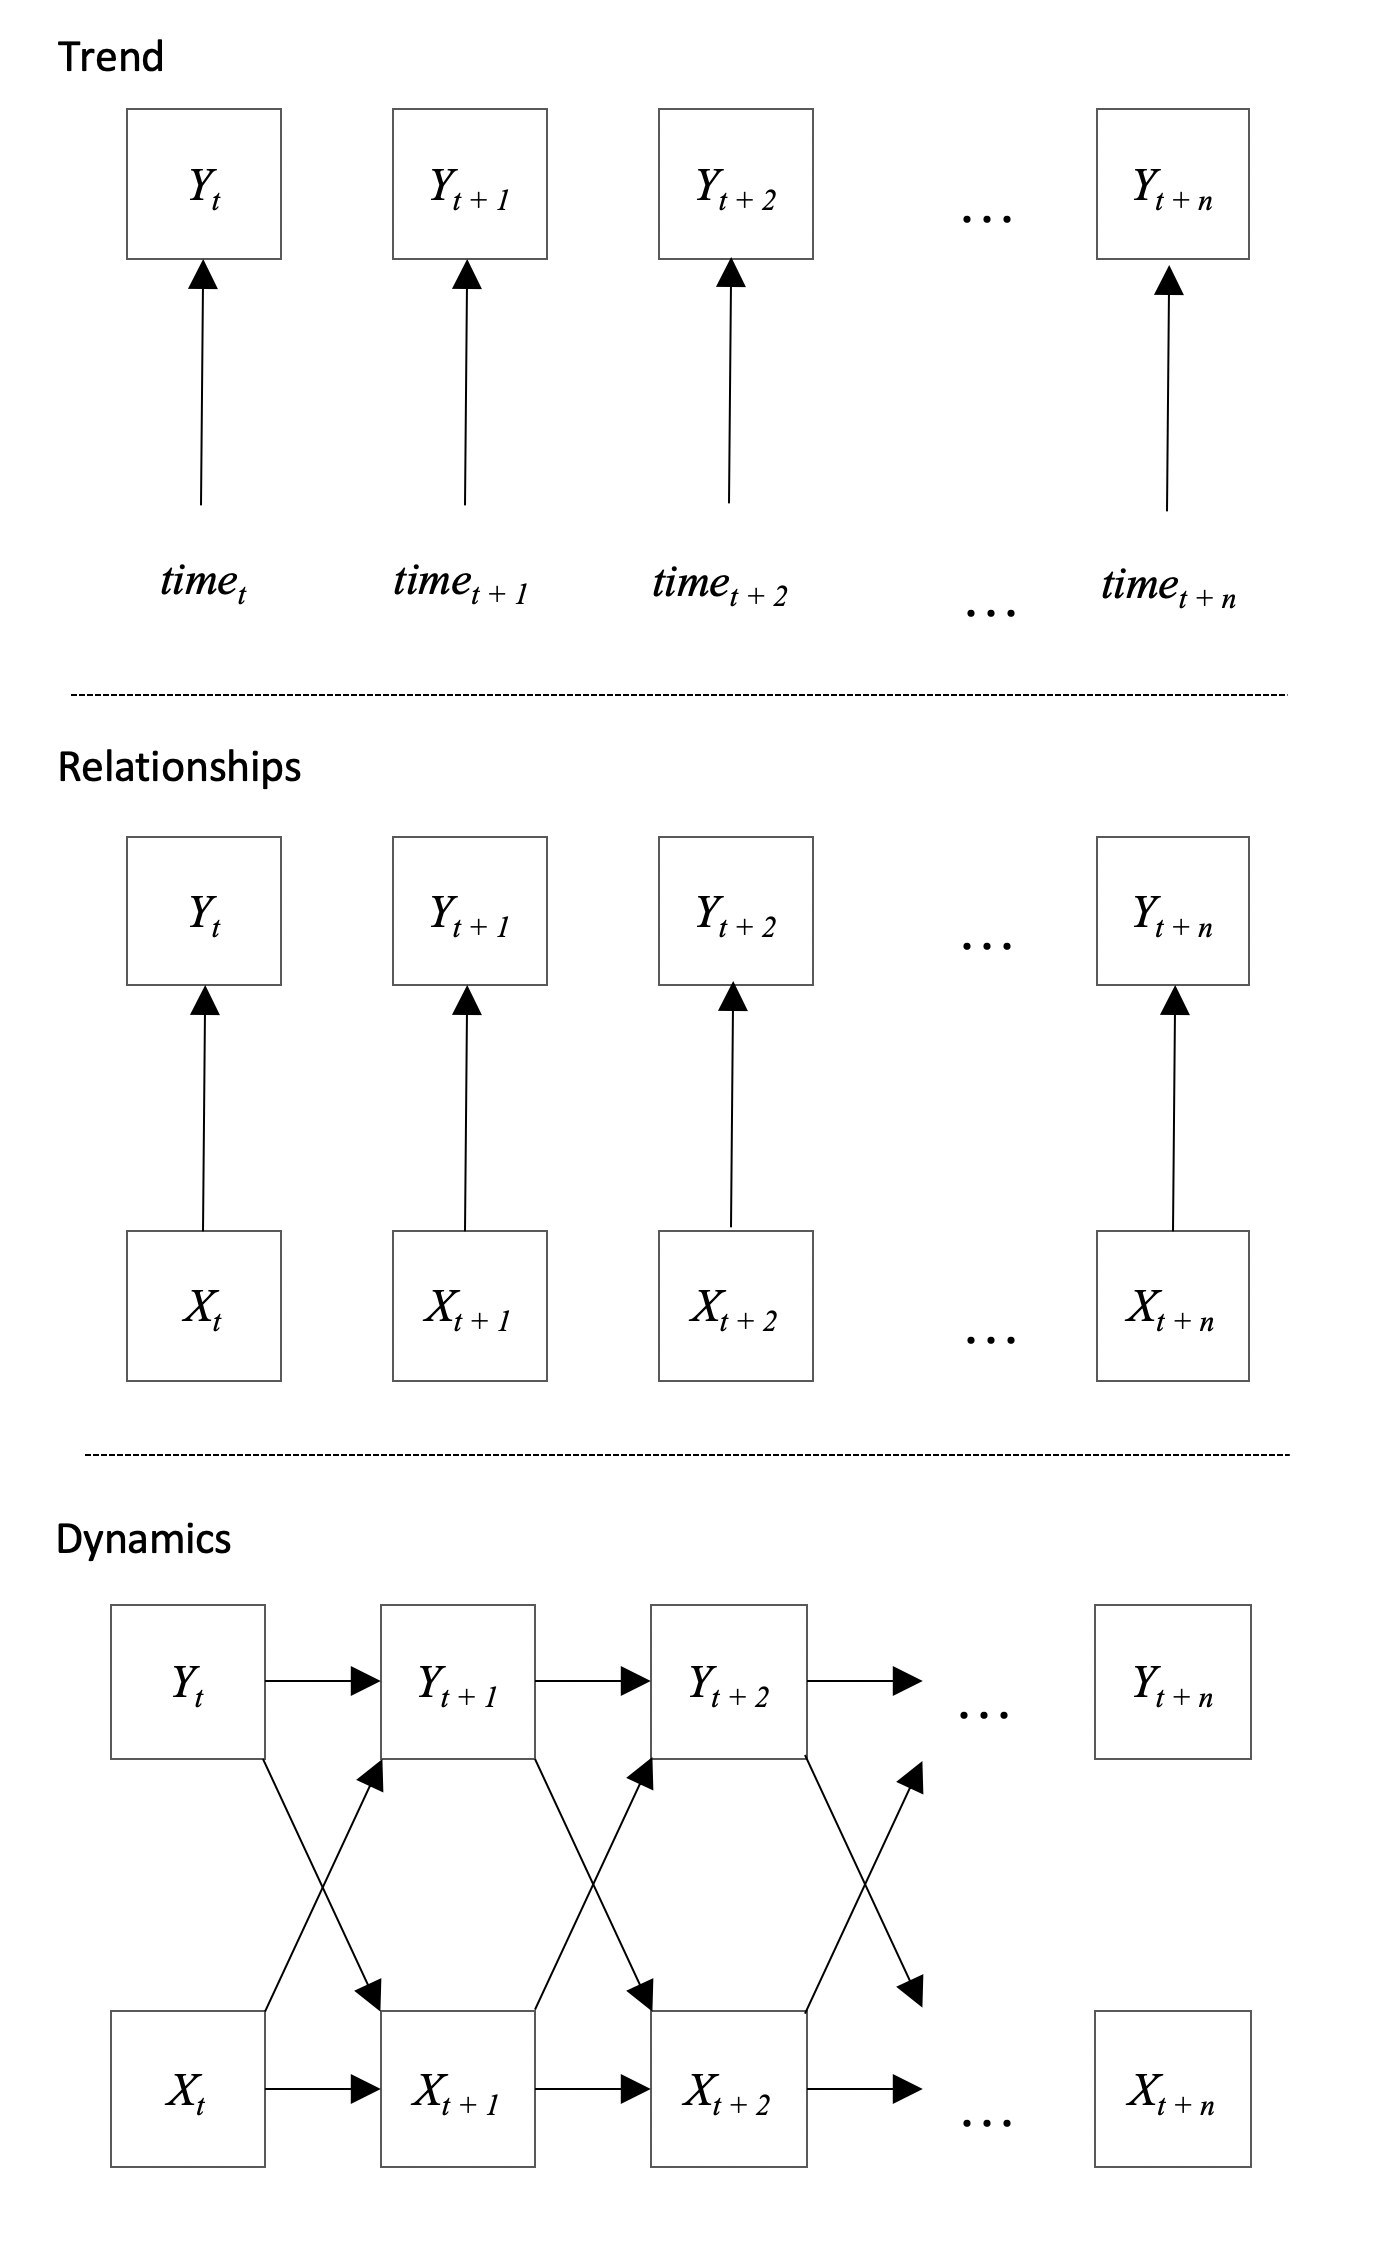
\includegraphics[width=4.66in]{figures/dynamics/framework} 

}

\caption{Common inference categories with models applied to longitudinal data.\label{framework_figure}}\label{fig:unnamed-chunk-6}
\end{figure}

\hypertarget{trend}{%
\section{Trend}\label{trend}}

Made popular in the organizational literature by Bliese and Ployhart
(2002) and Chan (1998), trend inferences represent a class of thinking
where researchers create an index of time and relate it to their
response variable. The first panel of Figure \ref{framework_figure}
shows a box-and-arrow heuristic where time is related to an outcome,
\(y\), and ultimately the analyst is interested in a variety of
questions about trend and its correlates. Trend inferences have two
components: trend itself and level. For clarity, we discuss them
separately.

\hypertarget{component-1---trend}{%
\subsubsection{Component 1 - Trend}\label{component-1---trend}}

Does affect, in general, go up or down across time, or is its trajectory
relatively flat? Does trainee skill generally increase over the training
session? These are questions about trend, and these first two are
specifically about linear trend. It is also possible to explore how
variables bend or curve across time. Do newcomer perceptions of climate
increase and then plateau over time? Does the response time of a medical
team decrease with each successive case but then remain stable once the
team can no longer improve their coordination? These latter questions
concern curvilinear trajectories.

Trend has to do with the systematic direction or global shape of a
trajectory across time. If we put a variable on the \(y\)-axis and plot
its values against time on the \(x\)-axis, do the values tend to go up
or down over time? It can be thought of as the coarse-grained direction
of a trajectory. A positive trend indicates that, on average, we expect
the variable to increase over time and a negative trend indicates that
we expect the variable to decrease over time. Our first trend inference,
therefore, concerns the shape of the trajectory.

\begin{quote}
\begin{quote}
\textbf{Inference 1:} On average, there is a
positive/negative/curvilinear trend.
\end{quote}
\end{quote}

Regardless of the specific technique or model, most inferences start
with the average pattern (or relationship) and then move to variability,
the same applies here. After learning about the average trend across the
sample researchers then focus on trend variability. How much consistency
is there in the trend pattern? Do all trainees develop greater skill
across time? Is there variability in the trend of helping behaviors, or
counterproductive work behaviors over time?

\begin{quote}
\begin{quote}
\textbf{Inference 2:} Trend differs/does not differ across units.
\end{quote}
\end{quote}

Inferences one and two concern one variable, but they can also be
iterated across all observed variables. For example, we might discover
that -- on average -- affect and performance trends both decrease, but
there is greater variability across units in the affect trend. Or we
might learn that affect has a negative trend while performance has a
positive trend.

Correlating these trends between-units is the next inference.
Correlating indicates co-occuring patterns, where a large, positive,
between-unit correlation between affect and performance trends would
indicate that people with a positive affect trend (usually) have a
positive performance trend and people with a negative affect trend
(usually) have a negative performance trend.

Figure \ref{trend_correlation} shows the inuition behind this inference
with a set of graphs. In Panel A we plot affect and performance across
time for three individuals. Affect goes up while performance goes down
for person one, this pattern is reversed for person two, and person
three reports trendless affect and performance (i.e., zero trend). We
use different colors to label the trends for each person. The affect and
performance trends for person one are labeled with red lines, whereas
person two has green lines and person three has blue lines.

Panel B then maps those pairings onto a scatterplot that demonstrates
the between-unit relationship among affect and performance trends. For
example, person one has a positive affect trend and a negative
performance trend, so their value in Panel B goes on the bottom right,
whereas person two has the opposite pattern and therefore is placed on
the top left (where the performance trend is positive and the affect
trend is negative). Producing this bottom scatter plot tells us that the
between-unit association among affect and performance trends is
negative. That is, people with a positive affect trend are expected to
have a negative performance trend, people with a negative affect trend
are expected to have a positive performance trend, and people with an
affect trend of zero are expected to have a performance trend of zero.

\begin{center}

------------

Insert Figure \ref{trend_correlation} about here

------------

\end{center}

\begin{quote}
\begin{quote}
\textbf{Inference 3:} Between-unit trends correlate.
\end{quote}
\end{quote}

The final trend inference is about identifying covariates or predictors
of trend. Does gender predict depletion trends? Does the trend in unit
climate covary with between-unit differences in leader quality?

Figure \ref{trend_covariate} demonstrates the inference in a plot. We
graph affect across time for six employees, and these employees differ
by job type. The first three individuals work in research and
development, whereas the final three work in sales. Affect trajectories
tend to decrease over time for employees in research and development,
whereas affect trajectories tend to increase for those in sales. An
individual's job type, then, gives us a clue to their likely affect
trend -- said formally, job type covaries with affect trend, such that
we expect individuals in sales to have positive affect trends and
individuals in research and development to have negative affect trends.
The expected trends are plotted as the thick blue lines.

\begin{center}

------------

Insert Figure \ref{trend_covariate} about here

------------

\end{center}

\begin{quote}
\begin{quote}
\textbf{Inference 4:} There are between-unit correlates of trend.
\end{quote}
\end{quote}

Note the difference between trend inferences three and four. Both are
between unit, but inference three is about co-occuring trend patterns
whereas inference four is about the relationship between trend and a
covariate/predictor. With respect to our examples, inference three says,
on average, if an individual has a positive affect trend then we expect
her to have a negative performance trend. Inference four says, on
average, if an individual is in research and development then we expect
him to have a negative affect trend.

\hypertarget{component-2---level}{%
\subsubsection{Component 2 - Level}\label{component-2---level}}

Researchers that explore trend also assess its predicted value at a
given time \(t\), and this second component is called level. Level is
almost always evaluated at the first or last observed time point --
e.g., What is the predicted level of the trainee skill trend at the
beginning of a training session? On average, what is the expected level
of the unit climate trend at the end of a two-week socialization
process? -- although researchers are free to asssess level at any \(t\).

\begin{quote}
\begin{quote}
\textbf{Inference 5:} On average, what is the expected level of the
\(y\) trend at time \(t\)?
\end{quote}
\end{quote}

After exploring the average trend level at a certain time we then move
to its variability. Trend lines have a beginning (or end) point, how
consistent do we expect that point to be? Is there variability in affect
trend starting level? Are there large between-unit differences in the
expected level of the performance trend at the last time point?

\begin{quote}
\begin{quote}
\textbf{Inference 6:} On average, there is variability in the expected
level of the \(y\) trend at time \(t\).
\end{quote}
\end{quote}

It is also possible to assess between unit correlations among level and
(a) trend in the same variable or (b) level or (c) trend in a different
variable. First consider a relationship among level and trend in the
same variable. On average, do people with low initial skill show
positive skill trends whereas people with high initial skill show
negative skill trends? Do organizations with high initial CWBs, on
average, tend to have negative CWB trends?

\begin{quote}
\begin{quote}
\textbf{Inference 7:} There is a between-unit correlation between trend
and level in \(y\).
\end{quote}
\end{quote}

Second, consider a between-unit correlation between level in one
variable and level in another. On average, do people with a low initial
performance also have low initial depletion (based on the initial levels
predicted by the performance and depletion trends)? Are organizations
with high initial turnover also expected, on average, to have high
burnout (based on the initial levels predicted by the turnover and
burnout trends)?

\begin{quote}
\begin{quote}
\textbf{Inference 8:} There is a between-unit correlation between level
of the \(x\) trend and level of the \(y\) trend at \(t\).
\end{quote}
\end{quote}

Finally, researchers are free to mix the inferences above and assess
whether levels in one variable covary with trend in another. Are people
with high initial voice (predicted by the voice trend) expected to have
negative satisfaction trends?

\begin{quote}
\begin{quote}
\textbf{Inference 9:} There is a between-unit correlation between the
level of the \(x\) trend at time \(t\) and the trend in \(y\).
\end{quote}
\end{quote}

A note on phrasing. The inferences we explored in this section have to
do with correlating levels and trends, where a statement like
\enquote{affect and performance trends covary between-units, such that
people with a negative affect trend have a positive performance trend}
is appropriate. There is a less precise phrase that is easy to fall into
-- and we have seen it used in our literature. Sometimes, researchers
will correlate trends and then state, \enquote{when affect decreases
performance goes up.} We urge researchers to avoid this second statement
because it is not clear if it refers to a static relationship about
trends or a dynamic statement about how trajectories move across time.
That is, the phrase \enquote{when affect decreases performance goes up}
could refer to between-unit correlated trends, but it could also mean
something like, \enquote{when affect decreases performance immediately
or subsequently goes up.} This second statement is far different and it
should not be used when an analysis only correlates trends or evokes
predictors of trend. Again, we urge researchers to phrase their
inferences as we have shown here.

\hypertarget{models}{%
\subsection{Models}\label{models}}

Trend is called the slope in the statistical modeling literature. That
is, when a researcher estimates a model to explore whether a variable
goes up or down over time she is estimating the trend coefficient. The
mean estimate refers to trend itself, whereas the variance estimate
refers to the trend variability across units. In the statistical
modeling literature these models are called growth-models or
growth-curves. Keep in mind, however, that researchers use the word
\enquote{change} informally to mean growth as well, so when you read a
theoretical discussion you may see words like \enquote{change} and
\enquote{increase} despite the researcher using a \enquote{growth}
model.

Broad theoretical discussions of growth are in Pitariu and Ployhart
(2010) and Ployhart and Vandenberg (2010) (keep in mind that they call
growth \enquote{change}), whereas Bliese and Ployhart (2002) describe
actual growth-curve analysis. Growth curves are a core topic in
developmental psychology, so there are many great articles and textbooks
to read from their field. See Grimm, Ram, and Estabrook (2016) and
Singer, Willett, and Willett (2003) for two great textbooks on growth
curve modeling, and McArdle and Epstein (1987) for an empirical
discussion. Two straight-forward empirical examples in our own field are
in Dunford et al. (2012) and Hülsheger (2016).

\begin{figure}
\centering
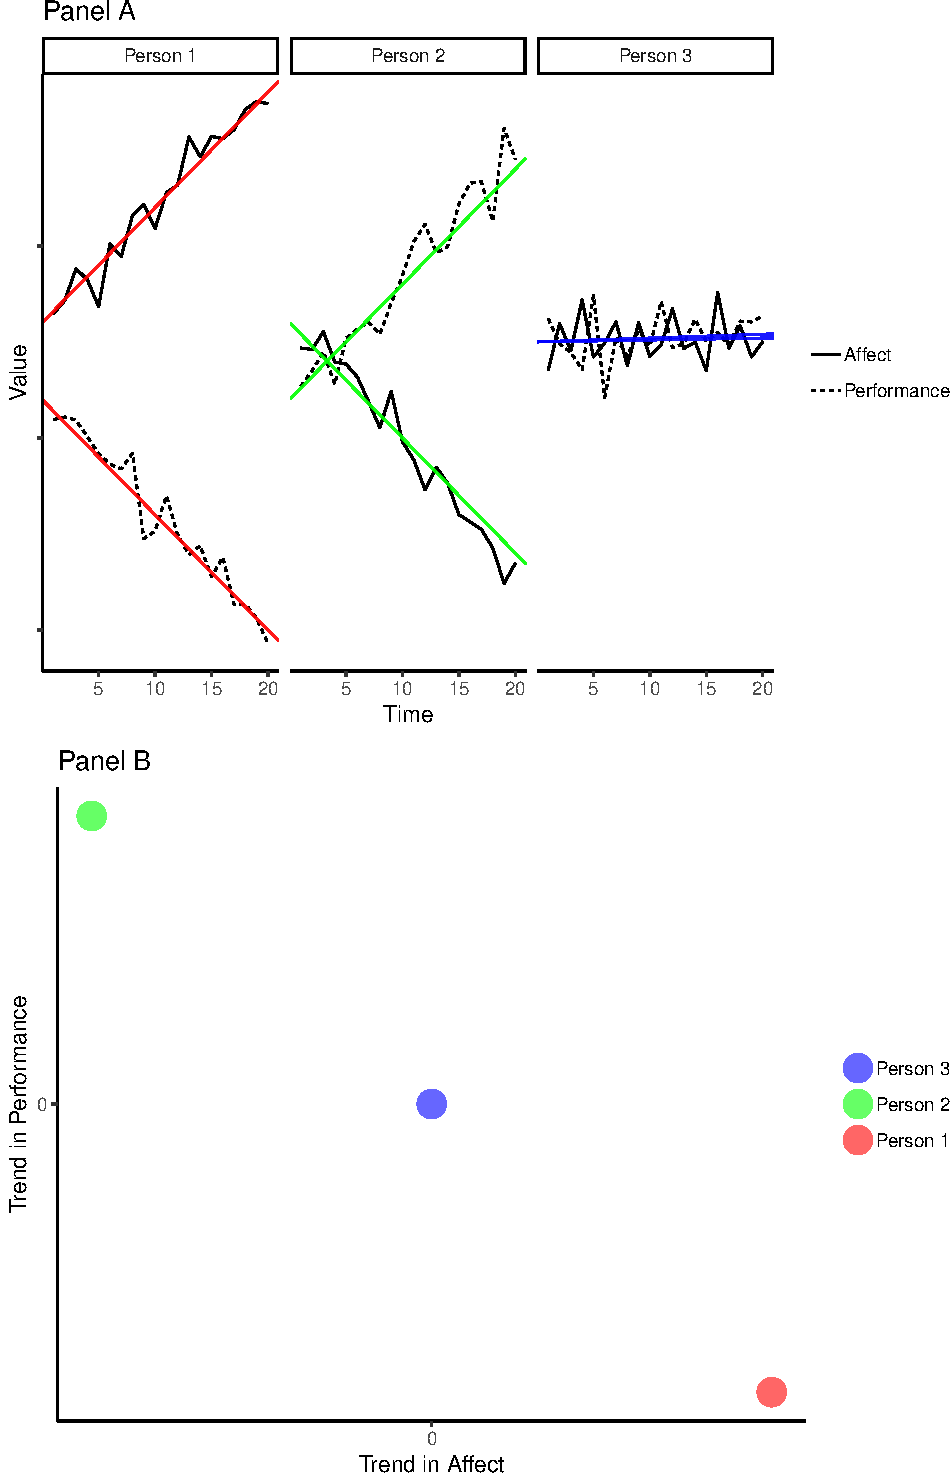
\includegraphics{figures/unnamed-chunk-10-1.pdf}
\caption{\label{fig:unnamed-chunk-10}Between-unit correlation of trend in
affect and performance.\label{trend_correlation}}
\end{figure}

\begin{figure}
\centering
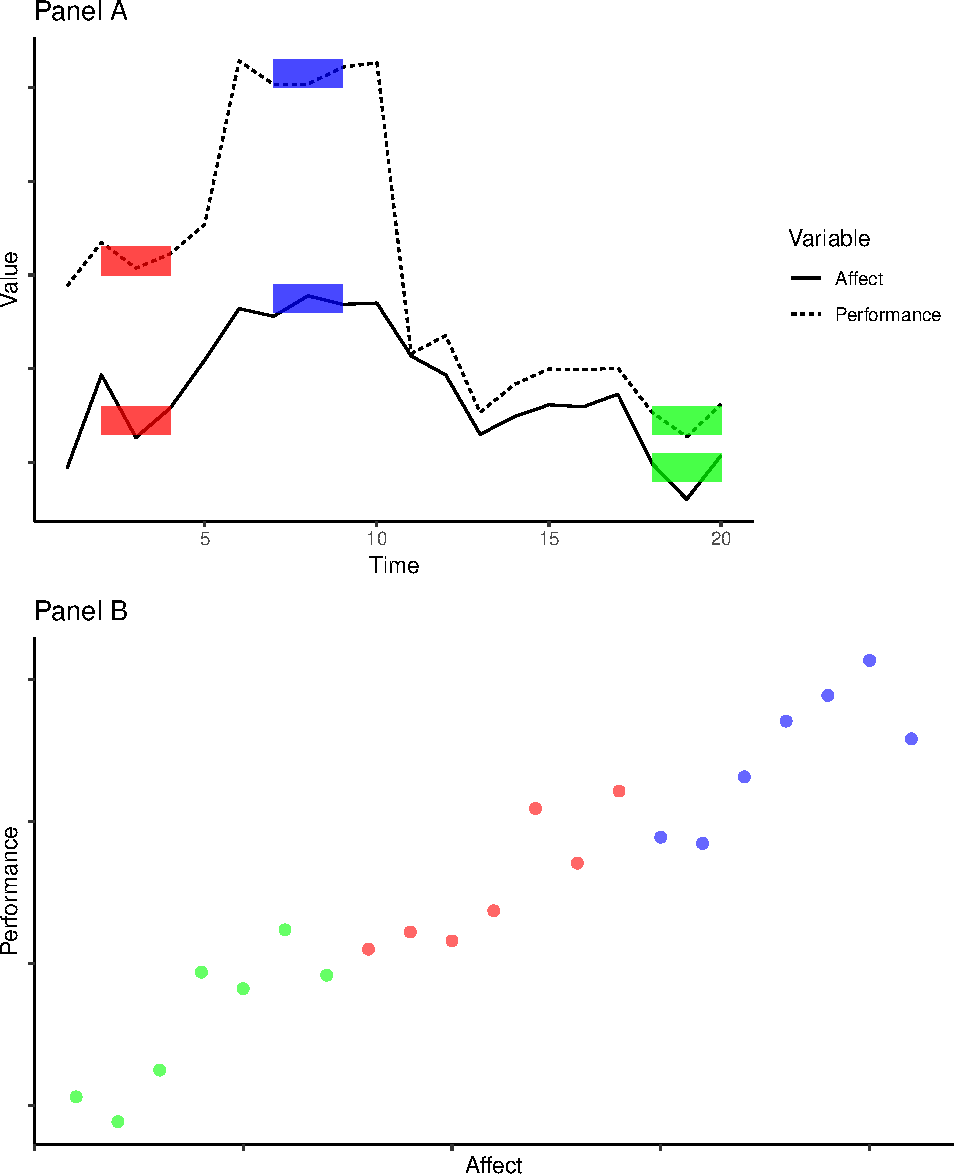
\includegraphics{figures/unnamed-chunk-11-1.pdf}
\caption{\label{fig:unnamed-chunk-11}Job type as a covariate of affect
trend.\label{trend_covariate}}
\end{figure}

\hypertarget{relationships}{%
\section{Relationships}\label{relationships}}

One of the most common inferences in our literature is to explore
between-unit relationships over time. The second panel of Figure
\ref{framework_figure} shows a relationships heuristic. A predictor is
concurrently related to a response variable at each time point and the
relationship is typically constrained to equality or is averaged over
time. Essentially, the inference compiles single-moment between-unit
correlations. For example, we assess the correlation between, say, OCBs
and depletion at time one, again and times two and three, and then
ultimately take the average of each individual correlation.

Questions about static relationships over time take the following forms.
What is the relationship between helping behaviors and incivility? Does
burnout predict turnover intention? Is unethical behavior related to
self-control?

Figure \ref{relation_tvc} shows the inuition of the inference with data.
Panel A plots affect and performance trajectories for three people. The
red circles in Panel A highlight each individual's affect and
performance values at time point six. Given that we have three people at
time point six, we can calculate a correlation between affect and
performance at that moment (granted, it is a small sample). The
calculated coefficient is then graphed in Panel B with another red
circle. At time point six, the correlation between affect and
performance across people is large and positive.

\begin{center}

------------

Insert Figure \ref{relation_tvc} about here

------------

\end{center}

Panel B also shows correlation coefficients for the rest of the time
points. Often these correlations are either averaged over time or
constrained to be equal. Again, this inference is one of the most common
inferences in our literature -- when a researcher uses a time-varying
covariates, hierarchical linear, random-coefficient, or multi-level
model on longitudinal data to explore concurrent relationships among one
or more variables (and they are not analyzing trend) they are making
this inference.

\begin{quote}
\begin{quote}
\textbf{Inference 1:} On average, what is the relationship between \(x\)
and \(y\) between-units? (Typically constrained to be equal over time or
averaged over time).
\end{quote}
\end{quote}

The first relationships inference emphasizes the expected average. As
with the trend inferences, the next question is to examine variability
in that estimated relationship across the sample. How consistent across
the sample is the relationship between distractions and fatigue? Is
there variability in the relationship between emotions and volunteering
behaviors?

\begin{quote}
\begin{quote}
\textbf{Inference 2:} There is variability in the between-unit
relationship among \(x\) and \(y\).
\end{quote}
\end{quote}

\hypertarget{models-1}{%
\subsection{Models}\label{models-1}}

Time-varying covariates (tvc) analysis is the workhorse behind
relationship inferences. A discussion of tvc models is in Schonfeld and
Rindskopf (2007) and Finch, Bolin, and Kelley (2016). Relatively
straight-forward empirical examples are in Barnes, Schaubroeck, Huth,
and Ghumman (2011) and Chi, Chang, and Huang (2015).

\begin{figure}
\centering
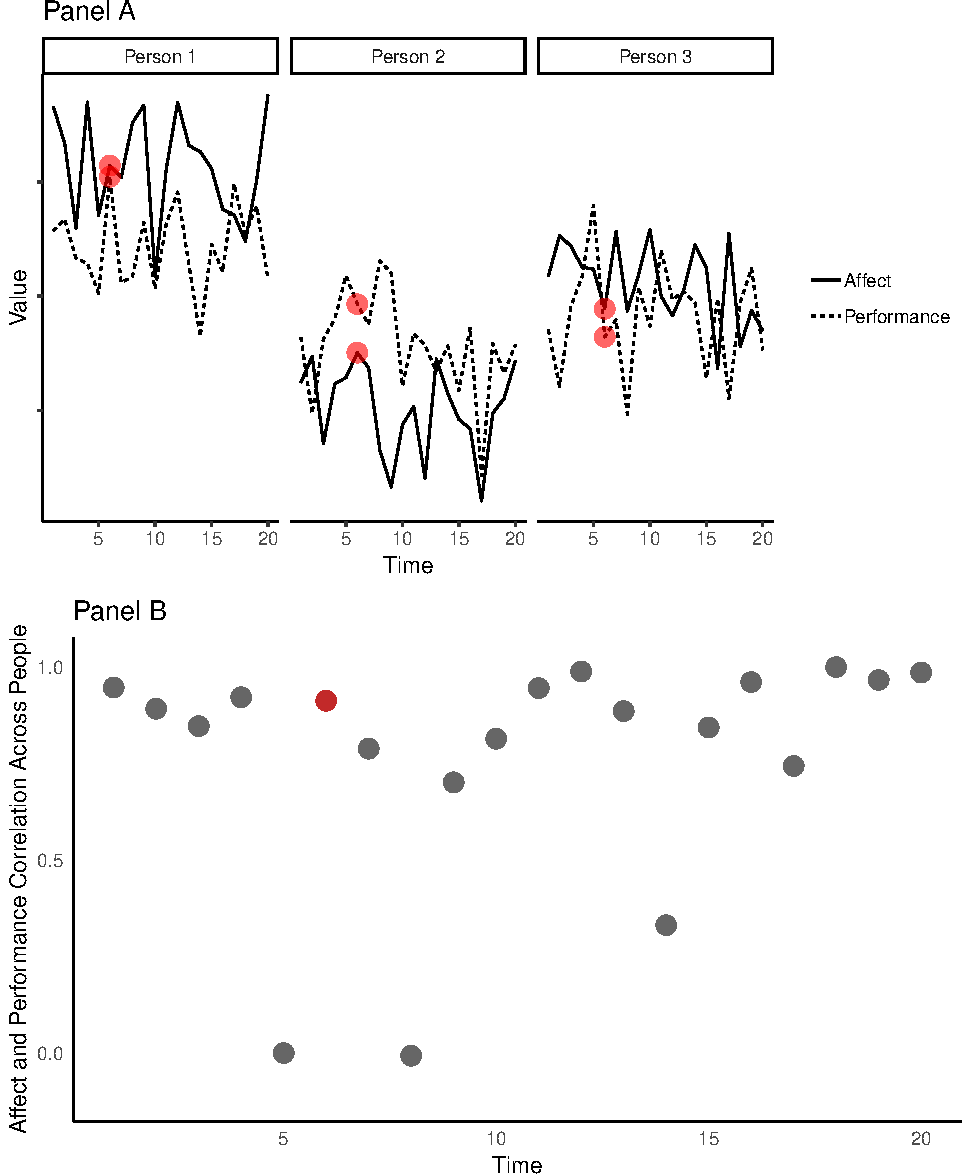
\includegraphics{figures/unnamed-chunk-14-1.pdf}
\caption{\label{fig:unnamed-chunk-14}Relating affect to performance across
units over time. The red circles demonstrate the between unit
correlation at time point six. A typical time-varying covariates model
constrains the correlation to be equivalent across time. Here, the
relationship is unconstrained at each time point.\label{relation_tvc}}
\end{figure}

\hypertarget{dynamics}{%
\section{Dynamics}\label{dynamics}}

Dynamics refers to a specific branch of mathematics, but the term is
used in different ways throughout our literature. It is used informally
to mean \enquote{change}, \enquote{fluctuating,} \enquote{volatile,}
\enquote{longitudinal,} or \enquote{over time} (among others), whereas
formal definitions are presented within certain contexts. Wang (2016)
defines a dynamic \emph{model} as a \enquote{representation of a system
that evolves over time. In particular it describes how the system
evolves from a given state at time \emph{t} to another state at time
\emph{t + 1} as governed by the transition rules and potential external
inputs} (p.~242). Vancouver, Wang, and Li (2018) state that dynamic
\emph{variables} \enquote{behave as if they have memory; that is, their
value at any one time depends somewhat on their previous value}
(p.~604). Finally, Monge (1990) suggests that in dynamic
\emph{analyses}, \enquote{it is essential to know how variables depend
upon their own past history} (p.~409). In this section we discuss a
number of inferences couched in the idea that the past constrains future
behavior.

Does performance relate to itself over time? Do current helping
behaviors depend on prior helping behaviors? Does unit climate
demonstrate self-similarity across time? Does income now predict income
in the future? These are questions about the relationship of a single
variable with itself over time -- does it predict itself at each
subsequent moment? Is it constrained by where it was in the past?

Panel A of Figure \ref{dynamics_figure} shows the concept with a
box-and-arrow diagram. \(y\) predicts itself across every moment -- it
has self-similarity and its value now is constrained by where it was a
moment ago. In our diagram we show that \(y\) at time \(t\) is related
to \(y\) at time \(t + 1\). In other words, we posit that \(y\) shows a
lag-one relationship, where \(y\) is related to its future value one
time step away. Researchers are of course free to suggest any lag amount
that they believe captures the actual relationship. Note that the
statistical term to capture self-similarity or memory is called
autoregression.

\begin{quote}
\begin{quote}
\textbf{Inference 1:} On average, there is self-similarity
(autoregression) in \(y\); \(y\) relates to itself across time.
\end{quote}
\end{quote}

\begin{center}

------------

Insert Figure \ref{dynamics_figure} about here

------------

\end{center}

As before, after exploring the expected average we turn to variability.
How consistent are the self-similarity relationships? Are there
between-unit differences in autoregression in, for example, employee
voice? Do we expect a large variance in the autoregression of helping
behaviors?

\begin{quote}
\begin{quote}
\textbf{Inference 2:} There is variability in the expected
autoregression of \(y\).
\end{quote}
\end{quote}

The next inference is about relating a predictor to our response
variable while it still retains memory. Panel B of Figure
\ref{dynamics_figure} shows a box-and-arrow diagram: \(y\) is predicted
by concurrent values of \(x\) but it also retains self-similarity. This
model is therefore said to partial prior \(y\): it examines the
concurrent relationship between \(x\) and \(y\) while statistically
partialling values of \(y\) at \(t - 1\), or statistically accounting
for \(y\) at the prior moment.

Our literature has converged on calling this kind of relationship
\enquote{change} because it emphasizes the difference between \(y\) now
and where it was in the past. The association asks how current \(x\)
relates to the difference between \(y\) now and its immediately prior
value. How does affect relate to change in performance? Does depletion
covary with change in OCBs? Note that change can be construed from any
prior time point (baseline, the prior time point, \(t-3\)); our
literature commonly emphasizes lag-one change.

\begin{quote}
\begin{quote}
\textbf{Inference 3:} On average, concurrent \(x\) relates to change in
\(y\).
\end{quote}
\end{quote}

The analyst is also free to assess variability in the expected change
relationship.

\begin{quote}
\begin{quote}
\textbf{Inference 4:} There is variability in the expected change
relationship between \(x\) and \(y\).
\end{quote}
\end{quote}

Change relationships do not have to be concurrent. Panel C of Figure
\ref{dynamics_figure} shows concurrent relationships as we saw above but
it also includes lags from the predictor to the outcome. \(y\) retains
memory, but it is predicted by both concurrent and prior values of
\(x\). Typically, we call these cross-lag relationships.

Questions about lag-one change relationships take the following forms.
Does affect predict subsequent performance change? Do prior
counterproductive work behaviors relate to current incivility change?
Does metacognition predict subsequent exploratory behavior change? Of
course, researchers can also explore longer lags by relating predictors
to more distal outcomes.

\begin{quote}
\begin{quote}
\textbf{Inference 5:} On average, there is a cross-lag relationship of
change, where \(x\) relates to the change in \(y\) at a different point
in time.
\end{quote}
\end{quote}

Again, typically researchers explore variability after assessing the
average estimate.

\begin{quote}
\begin{quote}
\textbf{Inference 6:} There is variability in the expected cross-lag
relationship of change.
\end{quote}
\end{quote}

\hypertarget{extensions}{%
\subsection{Extensions}\label{extensions}}

We described a simple set of inferences above, but the ideas generalize
to more complex dynamics as well. Often researchers are interested in
reciprocal relationships, where \(x\) influences subsequent \(y\), which
then goes back to influence \(x\) at the next time point. Said formally,
\(x_t\) influences \(y_{t+1}\), which then influences \(x_{t+2}\). Said
informally, current performance influences subsequent self-efficacy,
which then influences performance on the next trial. These inferences
are no different than what we saw above -- they are cross-lag
predictions -- all we did was add more of them. Panel D of Figure
\ref{dynamics_figure} shows reciprocal dynamics, where both \(x\) and
\(y\) show self-similarity and cross-lag relationships with one another.

Researchers typically posit a sequence of single cross-lag predictions
when they are interested in reciprocal dynamics. For example, Hardy III,
Day, and Steele (2018) explored reciprocal relationships among
performance and motivation (self-efficacy, metacognition, and
exploratory behavior). Their hypotheses include, (1) prior self-efficacy
negatively relates to subsequent exploratory behavior and (2) prior
exploratory behavior positively relates to subsequent self-efficacy
(among others). These single inferences are used in aggregate to make
conclusions about reciprocal influence.

The dynamic inferences shown here also generalize to systems of
variables where a researcher posits self-similarity and cross-lag
predictions across many variables. There could be reciprocal dynamics
between a set of variables like performance, self-efficacy, and affect,
or a sequence of influence between dyadic exchanges, performance, and
team perceptions: perhaps initial dyadic exchanges influence subsequent
team perceptions, which later influence performance. Following the
performance change, the structure of the task updates and this initiates
new dyadic exchanges. Once a researcher grasps the foundational ideas
presented here he or she is free to explore any number of complex
relationships.

Also notice that complex dynamics subsume the concept of mediation. It
is of course an important idea, but when we focus on systems of
variables and reciprocal dynamics we place our emphasis elsewhere. If
readers are interested in mediation we urge them to read one of the many
great papers on it (Maxwell \& Cole, 2007; Maxwell, Cole, \& Mitchell,
2011; Stone-Romero \& Rosopa, 2008).

\hypertarget{models-2}{%
\subsection{Models}\label{models-2}}

Wang et al. (2016) reviews many different types of dynamic models and,
although his paper will not provide readers will specific code it is an
excellent starting paper to observe the variety of dynamic models.

\begin{figure}

{\centering 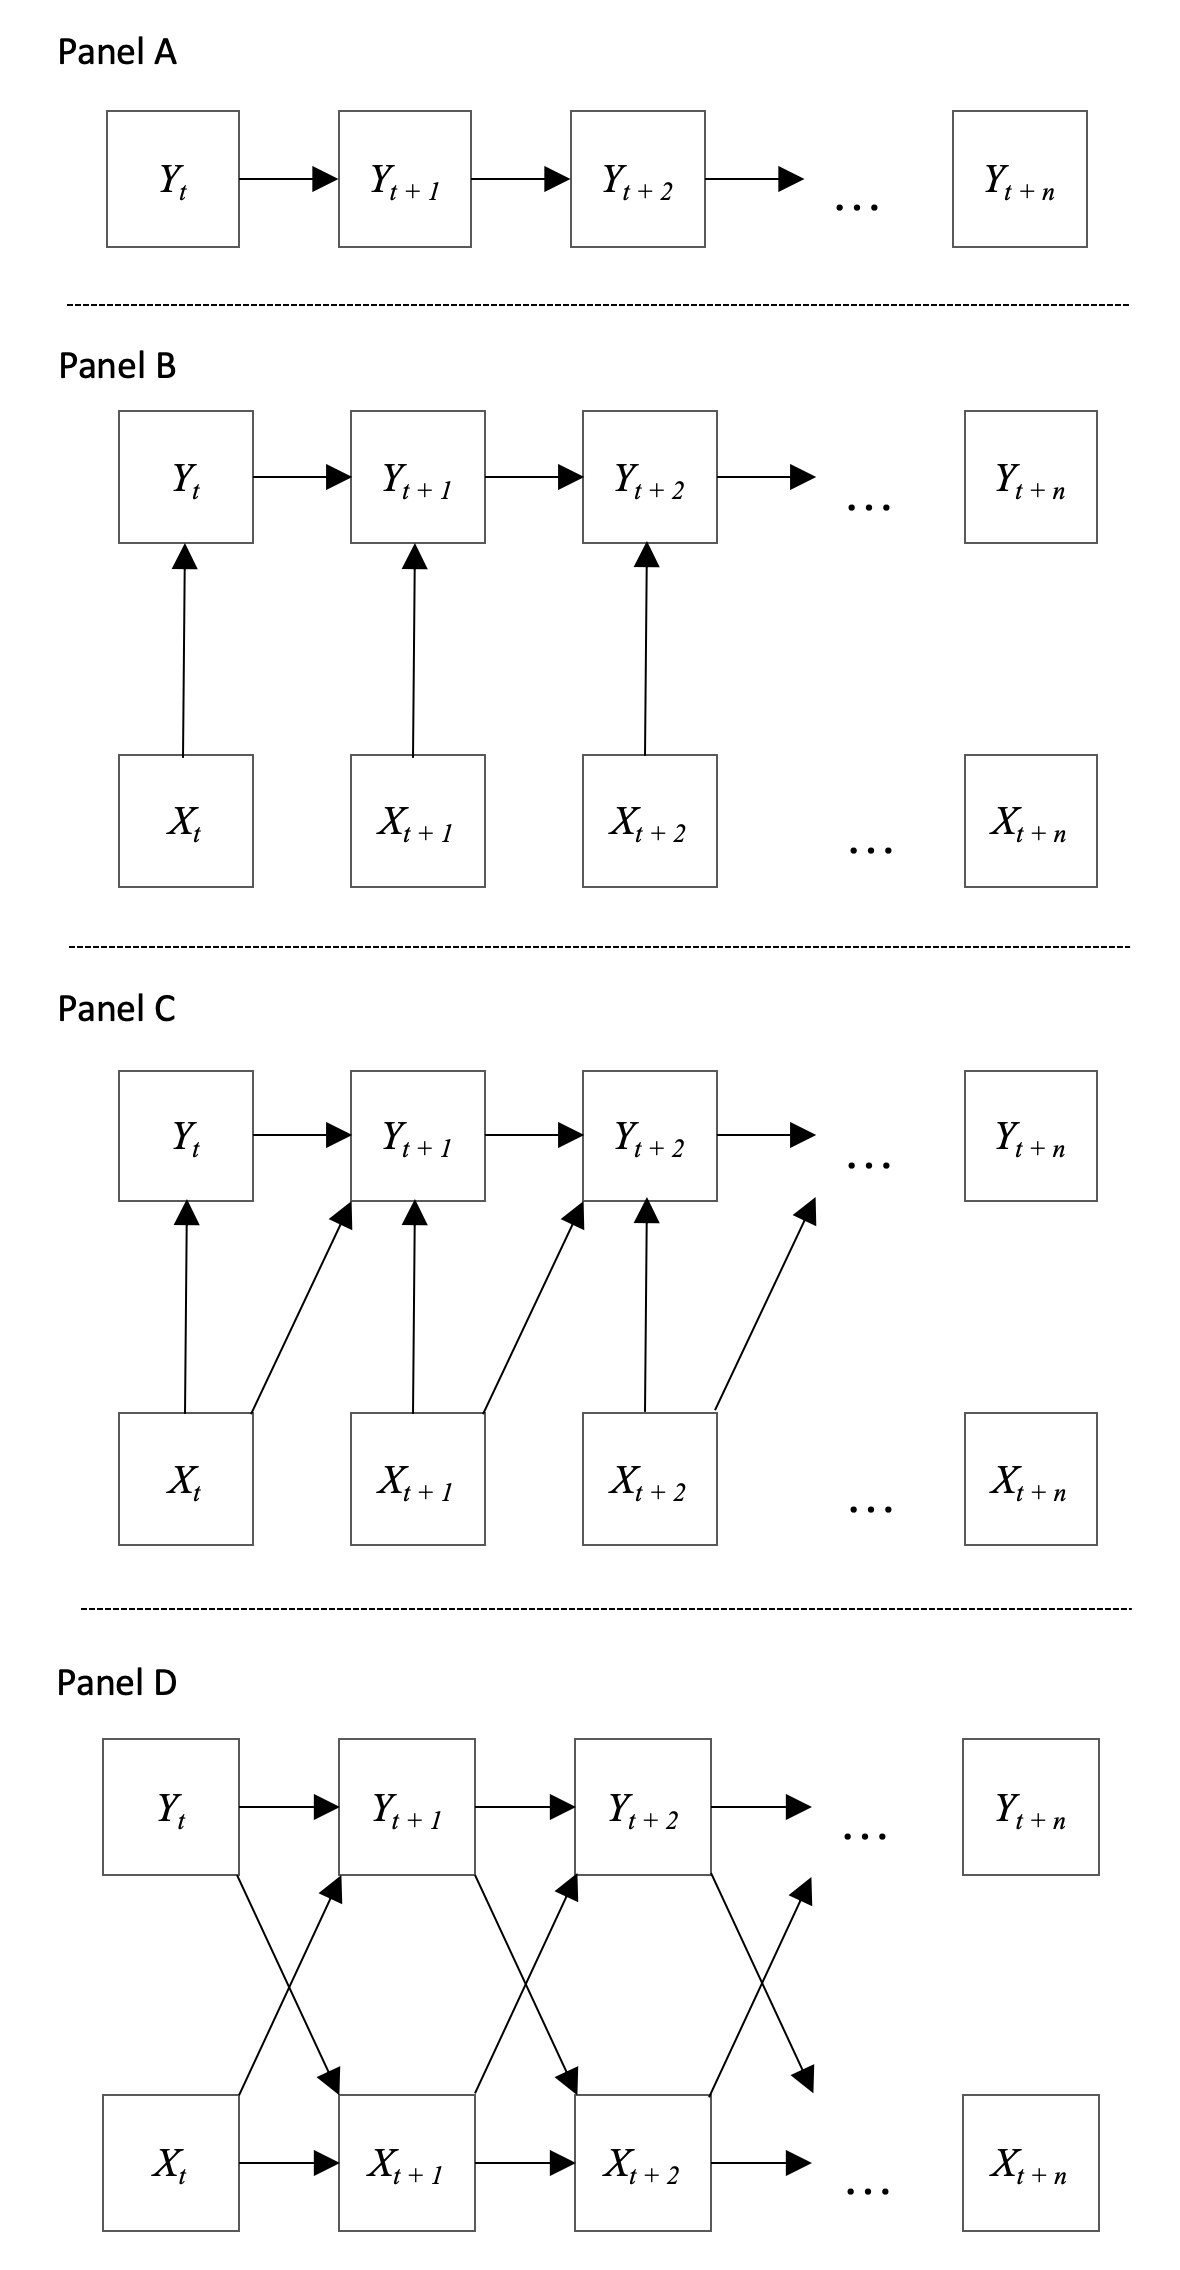
\includegraphics[width=3.93in]{figures/dynamics/dall} 

}

\caption{Univariate and bivariate dynamics adapted from DeShon (2012). Panel A shows self-similarity or autoregression in $Y$ across time. Panel B shows concurrent $X$ predicting change in $Y$. Panel C shows lagged change relationships. Panel D shows reciprocal dynamics between $X$ and $Y$.\label{dynamics_figure}}\label{fig:unnamed-chunk-16}
\end{figure}

\hypertarget{discussion}{%
\section{Discussion}\label{discussion}}

There are many different patterns to explore with longitudinal data
structures. What does performance look like over time? Does it
fluctuate? Is the trajectory consistent across people? What is its
initial or ending level? Does it show a growth pattern? Does that growth
pattern covary with another trend? Does it move across time in relation
to another variable? Does it show self-similarity or memory? Does it
show lagged relationships with other variables? Is it part of a
reciprocal system? In this paper we presented a framework that organizes
these inferences into a fundamental set. We discussed what the
inferences mean, how to pose questions and hypotheses about them, and
linked the inferences to appropriate statistical models. As our field
dives into within-person, dynamic, and process-oriented methods we hope
this paper helps researchers understand the spectrum of inferences that
they can explore with rich longitudinal data.

within person stuff

\newpage

\hypertarget{references}{%
\section{References}\label{references}}

\setlength{\parindent}{-0.5in}
\setlength{\leftskip}{0.5in}

\hypertarget{refs}{}
\leavevmode\hypertarget{ref-barnes_lack_2011}{}%
Barnes, C. M., Schaubroeck, J., Huth, M., \& Ghumman, S. (2011). Lack of
sleep and unethical conduct. \emph{Organizational Behavior and Human
Decision Processes}, \emph{115}(2), 169--180.

\leavevmode\hypertarget{ref-beal_esm_2015}{}%
Beal, D. J. (2015). ESM 2.0: State of the art and future potential of
experience sampling methods in organizational research. \emph{Annu. Rev.
Organ. Psychol. Organ. Behav.}, \emph{2}(1), 383--407.

\leavevmode\hypertarget{ref-bliese_growth_2002}{}%
Bliese, P. D., \& Ployhart, R. E. (2002). Growth modeling using random
coefficient models: Model building, testing, and illustrations.
\emph{Organizational Research Methods}, \emph{5}(4), 362--387.

\leavevmode\hypertarget{ref-chan1998conceptualization}{}%
Chan, D. (1998). The conceptualization and analysis of change over time:
An integrative approach incorporating longitudinal mean and covariance
structures analysis (lmacs) and multiple indicator latent growth
modeling (mlgm). \emph{Organizational Research Methods}, \emph{1}(4),
421--483.

\leavevmode\hypertarget{ref-chi_can_2015}{}%
Chi, N.-W., Chang, H.-T., \& Huang, H.-L. (2015). Can personality traits
and daily positive mood buffer the harmful effects of daily negative
mood on task performance and service sabotage? A self-control
perspective. \emph{Organizational Behavior and Human Decision
Processes}, \emph{131}, 1--15.

\leavevmode\hypertarget{ref-deshon_multivariate_2012}{}%
DeShon, R. P. (2012). Multivariate dynamics in organizational science.
\emph{The Oxford Handbook of Organizational Psychology}, \emph{1},
117--142.

\leavevmode\hypertarget{ref-dunford_is_2012}{}%
Dunford, B. B., Shipp, A. J., Boss, R. W., Angermeier, I., \& Boss, A.
D. (2012). Is burnout static or dynamic? A career transition perspective
of employee burnout trajectories. \emph{Journal of Applied Psychology},
\emph{97}(3), 637--650.
doi:\href{https://doi.org/http://dx.doi.org.proxy2.cl.msu.edu/10.1037/a0027060}{http://dx.doi.org.proxy2.cl.msu.edu/10.1037/a0027060}

\leavevmode\hypertarget{ref-finch2016multilevel}{}%
Finch, W. H., Bolin, J. E., \& Kelley, K. (2016). \emph{Multilevel
modeling using r}. Crc Press.

\leavevmode\hypertarget{ref-grimm_growth_2016}{}%
Grimm, K. J., Ram, N., \& Estabrook, R. (2016). \emph{Growth modeling:
Structural equation and multilevel modeling approaches}. Guilford
Publications.

\leavevmode\hypertarget{ref-hardy_interrelationships_2018}{}%
Hardy, J. H., Day, E. A., \& Steele, L. M. (2018). Interrelationships
Among Self-Regulated Learning Processes: Toward a Dynamic Process-Based
Model of Self-Regulated Learning. \emph{Journal of Management},
0149206318780440.
doi:\href{https://doi.org/10.1177/0149206318780440}{10.1177/0149206318780440}

\leavevmode\hypertarget{ref-hardy2018}{}%
Hardy III, J. H., Day, E. A., \& Steele, L. M. (2018).
Interrelationships among self-regulated learning processes: Toward a
dynamic process-based model of self-regulated learning. \emph{Journal of
Management}, 0149206318780440.

\leavevmode\hypertarget{ref-hulsheger_dawn_2016}{}%
Hülsheger, U. R. (2016). From dawn till dusk: Shedding light on the
recovery process by investigating daily change patterns in fatigue.
\emph{Journal of Applied Psychology}, \emph{101}(6), 905--914.
doi:\href{https://doi.org/http://dx.doi.org.proxy2.cl.msu.edu/10.1037/apl0000104}{http://dx.doi.org.proxy2.cl.msu.edu/10.1037/apl0000104}

\leavevmode\hypertarget{ref-ilgen_computational_2000}{}%
Ilgen, D. R., \& Hulin, C. L. (2000). \emph{Computational modeling of
behavior in organizations: The third scientific discipline.} American
Psychological Association.

\leavevmode\hypertarget{ref-jones_baby_2016}{}%
Jones, K. P., King, E. B., Gilrane, V. L., McCausland, T. C., Cortina,
J. M., \& Grimm, K. J. (2016). The baby bump: Managing a dynamic stigma
over time. \emph{Journal of Management}, \emph{42}(6), 1530--1556.

\leavevmode\hypertarget{ref-judge_what_2014}{}%
Judge, T. A., Simon, L. S., Hurst, C., \& Kelley, K. (2014). What I
experienced yesterday is who I am today: Relationship of work
motivations and behaviors to within-individual variation in the
five-factor model of personality. \emph{Journal of Applied Psychology},
\emph{99}(2), 199.

\leavevmode\hypertarget{ref-kozlowski_work_2003}{}%
Kozlowski, S. W., \& Bell, B. S. (2003). Work groups and teams in
organizations. \emph{Handbook of Psychology}, 333--375.

\leavevmode\hypertarget{ref-lanaj_when_2016}{}%
Lanaj, K., Johnson, R. E., \& Wang, M. (2016). When lending a hand
depletes the will: The daily costs and benefits of helping.
\emph{Journal of Applied Psychology; Washington}, \emph{101}(8), 1097.
Retrieved from
\url{http://search.proquest.com/docview/1813203845?pq-origsite=summon}

\leavevmode\hypertarget{ref-maxwell2007bias}{}%
Maxwell, S. E., \& Cole, D. A. (2007). Bias in cross-sectional analyses
of longitudinal mediation. \emph{Psychological Methods}, \emph{12}(1),
23.

\leavevmode\hypertarget{ref-maxwell2011bias}{}%
Maxwell, S. E., Cole, D. A., \& Mitchell, M. A. (2011). Bias in
cross-sectional analyses of longitudinal mediation: Partial and complete
mediation under an autoregressive model. \emph{Multivariate Behavioral
Research}, \emph{46}(5), 816--841.

\leavevmode\hypertarget{ref-mcardle_latent_1987}{}%
McArdle, J. J., \& Epstein, D. (1987). Latent Growth Curves within
Developmental Structural Equation Models. \emph{Child Development},
\emph{58}(1), 110--133.
doi:\href{https://doi.org/10.2307/1130295}{10.2307/1130295}

\leavevmode\hypertarget{ref-monge_theoretical_1990}{}%
Monge, P. R. (1990). Theoretical and analytical issues in studying
organizational processes. \emph{Organization Science}, \emph{1}(4),
406--430.

\leavevmode\hypertarget{ref-pitariu_explaining_2010}{}%
Pitariu, A. H., \& Ployhart, R. E. (2010). Explaining change: Theorizing
and testing dynamic mediated longitudinal relationships. \emph{Journal
of Management}, \emph{36}(2), 405--429.

\leavevmode\hypertarget{ref-ployhart_longitudinal_2010}{}%
Ployhart, R. E., \& Vandenberg, R. J. (2010). Longitudinal research: The
theory, design, and analysis of change. \emph{Journal of Management},
\emph{36}(1), 94--120.

\leavevmode\hypertarget{ref-rosen_who_2016}{}%
Rosen, C. C., Koopman, J., Gabriel, A. S., \& Johnson, R. E. (2016). Who
strikes back? A daily investigation of when and why incivility begets
incivility. \emph{Journal of Applied Psychology}, \emph{101}(11), 1620.

\leavevmode\hypertarget{ref-schonfeld2007hierarchical}{}%
Schonfeld, I. S., \& Rindskopf, D. (2007). Hierarchical linear modeling
in organizational research: Longitudinal data outside the context of
growth modeling. \emph{Organizational Research Methods}, \emph{10}(3),
417--429.

\leavevmode\hypertarget{ref-scott_multilevel_2011}{}%
Scott, B. A., \& Barnes, C. M. (2011). A multilevel field investigation
of emotional labor, affect, work withdrawal, and gender. \emph{Academy
of Management Journal}, \emph{54}(1), 116--136.

\leavevmode\hypertarget{ref-singer_applied_2003}{}%
Singer, J. D., Willett, J. B., \& Willett, J. B. (2003). \emph{Applied
longitudinal data analysis: Modeling change and event occurrence}.
Oxford university press.

\leavevmode\hypertarget{ref-stone2008relative}{}%
Stone-Romero, E. F., \& Rosopa, P. J. (2008). The relative validity of
inferences about mediation as a function of research design
characteristics. \emph{Organizational Research Methods}, \emph{11}(2),
326--352.

\leavevmode\hypertarget{ref-vancouver_translating_2018}{}%
Vancouver, J. B., Wang, M., \& Li, X. (2018). Translating Informal
Theories Into Formal Theories: The Case of the Dynamic Computational
Model of the Integrated Model of Work Motivation. \emph{Organizational
Research Methods}, 109442811878030.
doi:\href{https://doi.org/10.1177/1094428118780308}{10.1177/1094428118780308}

\leavevmode\hypertarget{ref-Wang2016}{}%
Wang, M., Zhou, L., \& Zhang, Z. (2016). Dynamic modeling. \emph{Annual
Review of Organizational Psychology and Organizational Behavior},
\emph{3}(1), 241--266.
doi:\href{https://doi.org/10.1146/annurev-orgpsych-041015-062553}{10.1146/annurev-orgpsych-041015-062553}


\end{document}
